\documentclass[10pt,a4paper]{book}
\usepackage[utf8]{inputenc}
\usepackage[english]{babel}
\usepackage{amsmath}
\usepackage{amsfonts}
\usepackage{amssymb}
\usepackage{wrapfig}
\usepackage{mathtools}
\usepackage{graphicx}
\usepackage{cancel}
\usepackage[left=2cm,right=2cm,top=2cm,bottom=2cm]{geometry}
\usepackage{physics}
\usepackage{multicol}
\usepackage{caption}
\usepackage{subcaption}
\author{Marco Biroli}
\title{Quantum Physics}
\begin{document}
\maketitle
\tableofcontents

\chapter{Hydrogen Atom.}
\section{Two Body problem and quantum mechanics.}
We consider two particles described by $\vec{r_1}, \vec{r_2}, \vec{p}_1, \vec{p}_2, m_1$ and $m_2$ that interact with a potential $V(\vec{r}_2 - \vec{r}_1)$. Then the Hamiltonian is given by:
\[
H = \frac{p_1^2}{2 m_1} + \frac{p_2^2}{2 m_2} + V(\vec{r_2} - \vec{r}_1)
\]
Now as usually done in classical physics we want to decompose the motion into the motion of the center of mass and a rotation around it. So we introduce:
\[
\vec{P} = \vec{p}_1 + \vec{p}_2,  \vec{R} = \frac{m_1 \vec{r_1} + m_2 \vec{r_2}}{m_1 + m_2}, \vec{r} = \vec{r_1} - \vec{r_2}, \vec{p} = \frac{m_2 \vec{p}_1 - m_1 \vec{p}_2}{m_1 + m_2}, M = m_1 + m_2, \mu = \frac{m_1 m_2}{m_1 + m_2}
\]
Then the Hamiltonian is re-written as:
\[
H = \underbrace{\frac{P^2}{2M}}_{H_{\text{CM}}} + \underbrace{\frac{p^2}{2\mu} + V(\vec{r})}_{H_\text{rel}}
\]
And the commutation relations are given by:
\[
[R_i, P_i] = i \hbar \delta_{ij}, [r_i, p_j] = i\hbar \delta_{ij}, [r_i, P_j] = 0, [R_i, p_j] = 0
\]
We immediately see that $[H, P] = 0$, this is a result of the invariance by translation of the problem. Hence $\vec{P}$ is a constant of the problem and $\vec{P}$ and $H$ share a common basis. The egein-values of the momentum of the center of mass are planes waves of the form:
\[
e^{i \vec{k} \cdot \vec{R}} \psi(\vec{r}) \quad \text{ and } \quad H_\text{rel} \psi(\vec{r}) = E \psi(\vec{r}) \Rightarrow E_\text{tot} = \frac{\hbar^2 k^2}{2 M} + E
\]
Now if we look at the specific case of the hydrogen atom since $m_p \gg m_e$ we have:
\[
\mu = \frac{m_e m_p}{m_e + m_p} = m_e \left[1 - \frac{m_e}{m_p}\right]
\]

\section{Central force movement.}
Say we have a potential of the form $V(\vec{r}) = V(r)$ then we want to solve the T.I.S.E.:
\[
\left[ \frac{p^2}{2m} + V(r) \right] \psi = E \psi \Leftrightarrow \left[ -\frac{\hbar^2}{2m} \frac{1}{r} \pdv[2]{}{r} r + \frac{L^2}{2m r^2} + V(r) \right]\psi = E \psi
\]
Remember also that $[L^2, H] = [L^2, L_i] = 0$, so $[\vec{L}, H] = 0$. So we can now look for solution that eigenstates of $L^2$ and $L_z$ which we know to be the spherical harmonics. So we decompose a given eigenstate in a radial component and a spherical harmonic component:
\[
R_l(r) Y_{l, m}(\theta, \varphi)
\]
Now plugging this into the T.I.S.E. we get:
\[
\left[ - \frac{\hbar^2}{2m} \frac{1}{r} \pdv[2]{}{r} r + \frac{l (l+1) \hbar^2}{2m r^2} + V(r) \right]R_l(r) = E R_l(r)
\]
And normalization gives:
\[\int_0^{+\infty} \int_{0}^\pi \int_{0}^{2\pi} r^2 \sin\theta\dd\theta \dd\varphi\dd r |R_l(r)|^2 |Y_{l,m}(\theta, \varphi)|^2 = \int_{0}^{+\infty} r^2 |R_l(r)|^2 \dd r = 
\]
Now to try and simplify the problem and reduce it to a 1D schrodinger equation we introduce a new function $u_l(r) = r R_l(r)$ we then have:
\[
\int_0^{+\infty} |u_l(r)|^2 = 1
\]
We also replace it in the T.I.S.E. which gives:
\[
\left[-\frac{\hbar^2}{2m} \pdv[2]{}{r} + \frac{l (l + 1) \hbar^2}{2m r^2} + V(r) \right] u_l(r) = E u_l(r)
\]
We see that we get a central force term plus a centrifugal term. The role of this centrifugal force is to make the potential diverge to infinity when $r$ goes to 0. A typical plot of this (for a coulomb potential) is as follows:
\begin{figure}[h!]
\centering
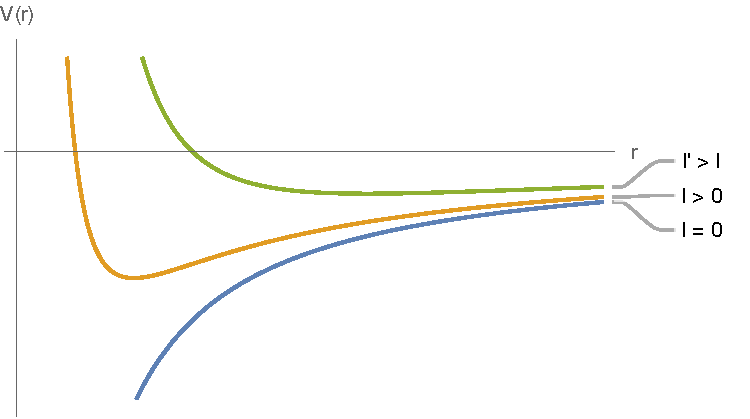
\includegraphics[width=0.6\textwidth]{graphs/center_force_potential}
\end{figure}

\subsection{Behavior close to the origin.}
We now write $u_l(r) \stackrel{r\to0}{\sim} C r^s$ and we assume that $V(r)$ does not go to infinity faster than $\frac{1}{r}$. Then we see that for the solution to be well defined we need the first two terms to cancel otherwise the solution diverges. So we get:
\[
-\frac{\hbar^2}{2m} s(s-1) + \frac{\hbar^2}{2m} l (l+1) = 0 \Leftrightarrow s = - l \lor s = l+ 1
\]
We see that the first solution is impossible if $l \neq 0$ since $u_l$ wouldn't be normalizable. It is also impossible when $l = 0$ because in that case $u_l(r) \sim c$ and so $R_l(r) \sim \frac{C}{r}$, but then $\Delta R_l = -4 \pi C \delta$ which is not a viable solution to the Schrodinger equation. So the only viable solution is $s = l+1$. So we now need to solve the following equation:
\[
\left[ - \frac{\hbar^2}{2m} \pdv[2]{}{r} + \frac{l(l+1) \hbar^2}{2m r^2} + V(r)\right] u_l(r) = E u_l(r) \quad \land \quad u_l(0) = 0
\]
We know that there are discrete energies solution to this problem and actually for the coulomb potential case the energies will be given by: $n' + l + 1 = n$. We call $n$ the principal quantum number.

\section{Hydrogen Atom.}
For the hydrogen atom the potential is given by: $V(r) = \frac{-q^2}{4\pi \varepsilon_0 r}$ to simplify the writing we introduce $e^2 = \frac{q^2}{4 \pi \varepsilon_0}$ so that $V(r) = - \frac{e^2}{r}$. Then the T.I.S.E. is given by:
\[
\left[ -\frac{\hbar^2}{2m} \pdv[2]{}{r} + \frac{l ( l + 1) \hbar}{2 m r^2} - \frac{e^2}{r} \right] u_l(r) = E u_l(r)
\]
We want to make the problem dimensionless so we introduce $a_0 = \frac{\hbar^2}{m e^2}= 0.53 \stackrel{\circ}{A}$ as a unit for length, $E_I = \frac{e^2}{2 a_0} = \frac{m^2 e^4}{2 \hbar^2} = 13.6 \text{ eV} $ as a unit for energy. We now introduce the dimensionless parameters $\rho = \frac{r}{a_0}$ and $\varepsilon = -\frac{E}{E_I}$ and plugging them in the T.I.S.E. we get:
\[
\left[ \dv[2]{}{\rho} - \frac{l(l+1)}{\rho^2} + \frac{2}{\rho} - \varepsilon \right] u_l(\rho) = 0
\]
When $\rho \to \infty$ the equation simplifies to something that gives $e^{\pm \sqrt{\varepsilon} \rho}$ the plus being non-normalizable we keep only the minus and we introduce a new variable: $u_l(\rho) = y_l(\rho) e^{-\sqrt{\varepsilon} \rho}$ and plugging this in and introducing $\lambda = \sqrt{\varepsilon}$ we get:
\[
\left[ \dv[2]{}{\rho} - 2\lambda \dv{}{\rho} + \left[\frac{2}{\rho} - \frac{l (l + 1)}{\rho^2} \right] \right] y_l = 0 \land y_l(0) = 0
\]
To solve this we pass by the series decomposition of $y_l$:
\[
y_l(\rho) = \rho^s \sum_{q = 0}^{\infty} c_q \rho^q \text{ with } s > 0 \text{ in order for } y_l(0) = 0
\]
Then the derivatives are given by:
\[
\dv{y_l(\rho)}{\rho} = \sum_{q = 0}^{+\infty} c_q \rho^{q + s - 1} (q + s) \land \dv[2]{y_l(\rho)}{\rho} = \sum_{q = 0}^{+\infty} c_q (q + s) (q + s - 1) e^{q + s - 2}
\]
Then plugging this into the differential equation and using the uniqueness of the series expansion we get the following recursion relation:
\[
c_q \left[ q (q + 2l + 1) \right] = 2 \left[(q+l)\lambda - 1 \right] c_{q-1} \Rightarrow \frac{c_q}{c_{q-1}} \stackrel{q \to \infty}{\sim} \frac{2\lambda}{q} \Rightarrow y_l(\rho) \stackrel{q \to \infty}{\sim} e^{2\lambda \rho}
\]
However if this was true then it would mean that $u_l(\rho) \stackrel{\rho \to \infty}{\sim} e^{\lambda \rho}$ which is impossible. Therefore it must be that $c_q$ terminates for a certain $n' \in \mathbb{N}$. Hence:
\[
(n' + 1 + l) \lambda - 1 = 0 \Rightarrow c_{n'+1} = 0
\]
Then the energy is given by:
\[
\varepsilon = \lambda^2 = \frac{1}{(n' + 1 + l)^2} \Leftrightarrow E = \frac{-E_I}{(n' + 1 + l)^2}
\]
Now note that the degeneracy of a given energy is given by the amount of ways we can write $n = n' + 1 + l$ changing $n'$ and $l$. So for $n$ given there are $n$ possible values that $l$ can take, for every $l$ there are $(2l +1)$ values that $m$ can take. So the degeneracy of a state of principal quantum number $n$ is given by:
\[
g_n = \sum_{l = 0}^{n-1} (2l + 1) = n^2
\]

\end{document}